\documentclass[11 pt]{article}
\usepackage{amsmath, amssymb, color, xcolor}
\usepackage{graphicx, wrapfig, float, caption, dsfont}
\usepackage{fullpage}
\usepackage[backref=page, hidelinks, colorlinks=true, citecolor=blue!60!black!100]{hyperref}
\usepackage{tikz}
\usetikzlibrary{arrows.meta, shapes}
\usepackage{caption, subcaption}
\usepackage{natbib} % gives us \citet: Author (year) and \citep: (Author; year)
\usepackage{authblk}

\newcommand{\plr}[1]{{\color{blue}\it #1}}
\newcommand{\jss}[1]{{\color{olive}\it #1}}
% \newcommand{\ddt}{\frac{d}{dt}}
\newcommand{\ddt}{\dot}
\newcommand{\ro}{{ro}}
\newcommand{\nro}{{\bar{r}o}}
\newcommand{\rno}{{r\bar{o}}}
\newcommand{\nrno}{{\bar{r}\bar{o}}}
\newcommand{\reachable}{\mathcal{R}}
\newcommand{\unobservable}{\bar{\mathcal{O}}}
\newcommand{\R}{\mathbb{R}}
\newcommand{\E}{\mathbb{E}}
\renewcommand{\P}{\mathbb{P}}
\newcommand{\pda}{\frac{\partial}{\partial A_{ij}}}
\newcommand{\ind}{\mathds{1}}

\DeclareMathOperator{\spn}{span}

\newtheorem{theorem}{Theorem}
\newtheorem{lemma}{Lemma}
\newtheorem{definition}{Definition}
\newtheorem{example}{Example}

\begin{document}

  \section{\emph{S. cerevisiae} galactose catabolism network}

  Yeast galactose catabolism is accomplished via a complex system of molecules including enzymes, transporters, and transcription factors. The GAL2 gene encodes a transporter than imports galactose into the cell cytoplasm. GAL1, GAL7, and GAL10 encode components of enzymes that act sequentially to metabolize the imported galactose. Furthermore, in \emph{S. cerevisiae} the enzyme encoding genes, GAL1, GAL7, and GAL10 are encoded within the same regulon (on the same chromosome and regulated by the same promoter), whereas GAL2 is encoded on a separate chromosome. The transcription factor produced by GAL4 binds to promoter of the regulon, inducing the expression of the enzymes. Another gene, MIG1, which is induced by the presence of glucose, encodes a repressor for the GAL regulon. MIG1 acts by repressing the GAL enzymes, as well as down regulating some of the GAL transcription factors, by repressing GAL4 and GAL3, but not acting on GAL80. MIG1 also represses the transporter GAL2.

   \begin{figure}
        \begin{center}
            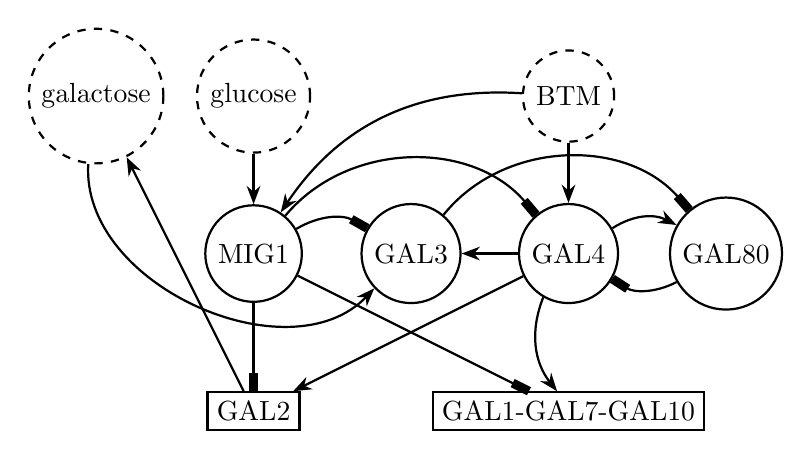
\begin{tikzpicture}
            \begin{scope}[every node/.style={circle,thick,draw}]
                \node (GAL3) at (2,0) {GAL3};
                \node (GAL4) at (4,0) {GAL4};
                \node[dashed] (BTM) at (4,2) {BTM};
                \node (GAL80) at (6,0) {GAL80};
                \node (MIG1) at (0,0) {MIG1};
                \node[shape=rectangle] (GAL2) at (0,-2) {GAL2};
                \node[shape=rectangle] (enzymes) at (4,-2) {GAL1-GAL7-GAL10};
                \node[dashed] (galactose) at (-2, 2) {galactose};
                \node[dashed] (glucose) at (0,2) {glucose};
            \end{scope}

            \begin{scope}[>={Stealth[black]},
                          every edge/.style={draw=black, thick}]
                 \path[->] (GAL4) edge[left] node {} (GAL3);
                 \path[->] (GAL4) edge[bend left] node {} (GAL80);
                 \path[->, >=Rectangle] (GAL3) edge[bend left=50] node {} (GAL80);
                 \path[->, >=Rectangle] (GAL80) edge[bend left] node {} (GAL4);
                 \path[->] (GAL4) edge[bend right] node {} (enzymes);
                 \path[->] (GAL4) edge[left] node {} (GAL2);
                 \path[->, >=Rectangle] (MIG1) edge[bend left] node {} (GAL3);
                 \path[->, >=Rectangle] (MIG1) edge[bend left=50] node {} (GAL4);
                 \path[->, >=Rectangle] (MIG1) edge node {} (enzymes);
                 \path[->, >=Rectangle] (MIG1) edge node {} (GAL2);
                 \path[->] (glucose) edge node {} (MIG1);
                 \path[->] (galactose) edge[bend right=70] node {} (GAL3);
                 \path[->] (GAL2) edge node {} (galactose);
                 \path[->] (BTM) edge node {} (GAL4);
                 \path[->] (BTM) edge[bend right] node {} (MIG1);
            \end{scope}
            \end{tikzpicture}
        \end{center}
        \caption{
          Yeast galactose catabolism transcription network.}
    \end{figure}

    \begin{align*}
      \dot{x}(t) &= \begin{bmatrix} 0 & + & 0 & - \\ 0 & 0 & - & - \\ - & + & 0 & 0 \\ 0 & 0 & 0 & 0 \end{bmatrix} \begin{bmatrix} \text{GAL3} \\ \text{GAL4} \\ \text{GAL80} \\ \text{MIG1} \end{bmatrix}(t) + \begin{bmatrix} + & 0 & 0 \\ 0 & 0 & + \\ 0 & 0 & 0 \\ 0 & + & + \end{bmatrix} \begin{bmatrix} \text{galactose} \\ \text{glucose} \\ \text{BTM} \end{bmatrix}(t) \\
        y(t) &= \begin{bmatrix} 0 & + & 0 & - \end{bmatrix} \vec{x}(t)
    \end{align*}
    In the above parameterization, $y(t)$, or the cumulative impact of transcriptional regulation on the expression of the GAL regulon, will either tend towards positive or negative infinity depending on the ratio of galactose to glucose, and the impact of the basal transcriptional machinery (BTM) on the components of the system.
    
    \subsection{Notes}
    \begin{itemize}
      \item The interaction strength between GAL4 and GAL80 can be altered via mutation. Furthermore, a mutation in GAL4 that decreases affinity can be compensated by a mutation in GAL80 \citep{li2010alterations, salmeron1990gal4, adhikari2014perturbation}.
      \item The galactose metablic network shows tremendous regulatory variation among different species of yeast \citep{lavoie2009rearrangements, martchenko2007transcriptional, dalal2016transcriptional, christensen2011unique, hartl2007induction, alam2013aspergillus}.
      \item GAL3 (a TF) is a paralog of GAL1 (enzyme), yet GAL3 no longer has any galactokinase activity. GAL1, however, can weakly regulate in place of GAL3.
    \end{itemize}


\bibliographystyle{plainnat}
\bibliography{krefs}

\end{document}

